\section{Backend}\label{sec:poc:backend}
\begin{figure}[ht]
  \centering
  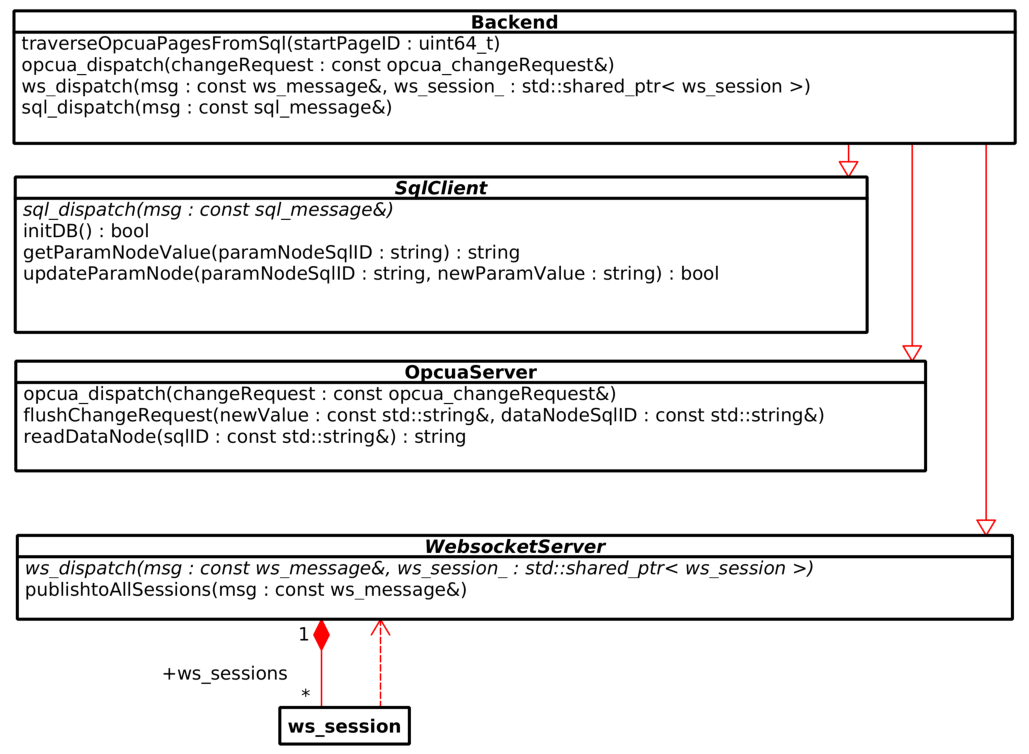
\includegraphics[width=\textwidth]{content/hauptteil/umsetzungPoC/backend/uml/overview.pdf}
  \caption{Klassediagramm Überblick Backend}
  \label{fig:backend:classDiag:overview}
\end{figure}
%beschreibung diagramm
%erwähnung datenaustausch zwischen basisklassen zu abgeleitetrer...(dispatcher.... )
  %endlich anzahl an fkt für daten backend -> basisklassen
  %pro basisklasse ein dispatcher im Backend (virtual) --> Verweis auf Kapitel
%erwähnung message klassen die geparsed wwerden


\subsection{WebsocketServer}
%kurze Erwähnung sinn der klasse
%datenaustausch zwischen WebsocketServer zu abgeleitetrer...(dispatcher.... ) (I/O)
\begin{figure}[ht]
  \centering
  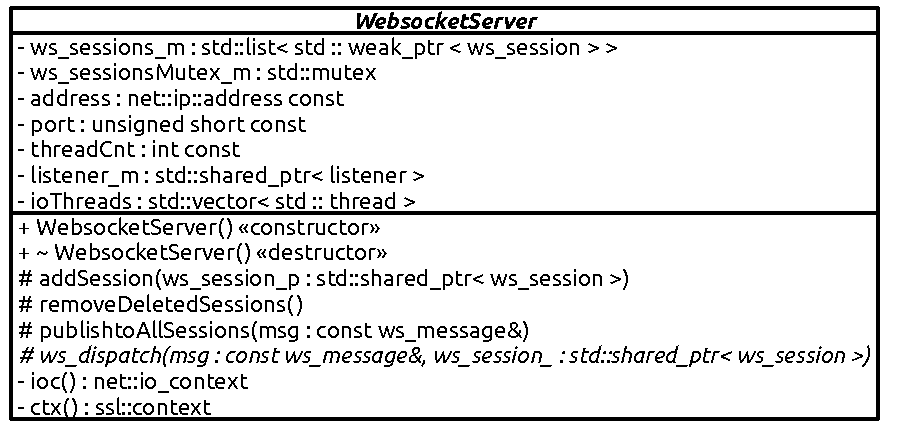
\includegraphics[width=\textwidth]{content/hauptteil/umsetzungPoC/backend/uml/classesOfOverview/WebsocketServer.pdf}
  \caption{Klassediagramm der Klasse WebsocketServer}
  \label{fig:backend:classDiag:WebsocketServer}
\end{figure}
%beschreibung msg klasse mit diagram
\begin{figure}[ht]
  \centering
  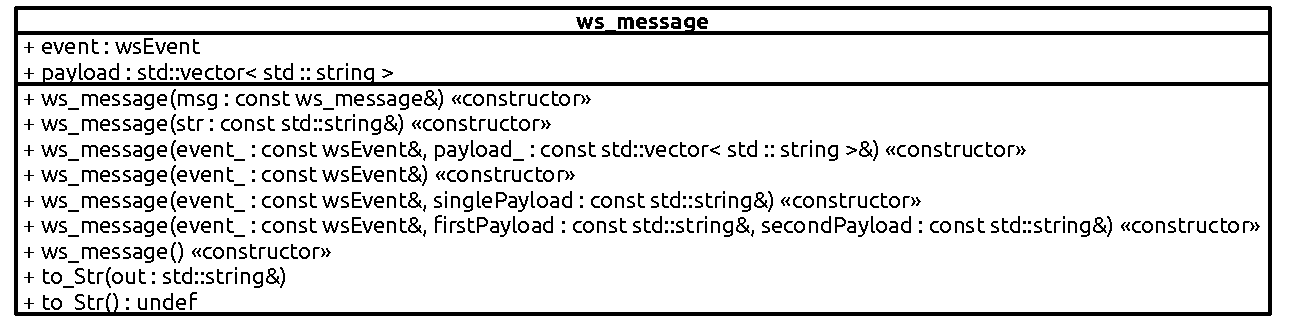
\includegraphics[width=\textwidth]{content/hauptteil/umsetzungPoC/backend/uml/classesOfOverview/ws_message.pdf}
  \caption{Klassediagramm der Klasse ws\_message}
  \label{fig:backend:classDiag:wsMsg}
\end{figure}
%dispatcher codeausschnitt
%beschreibung dispatcher
\subsection{SqlClient}
%kurze Erwähnung sinn der klasse
%datenaustausch zwischen SqlClient zu abgeleitetrer...(dispatcher.... ) (I/O)
\begin{figure}[ht]
  \centering
  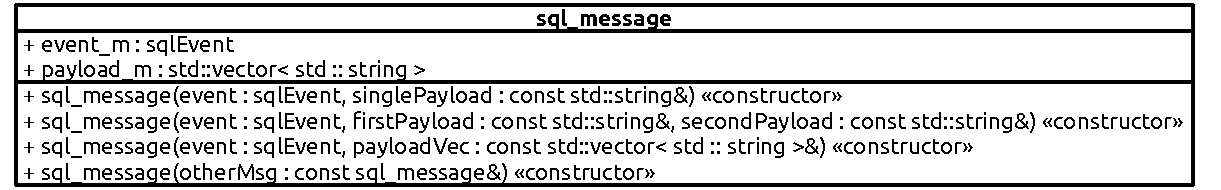
\includegraphics[width=\textwidth]{content/hauptteil/umsetzungPoC/backend/uml/classesOfOverview/sql_message.pdf}
  \caption{Klassediagramm der Klasse sql\_message}
  \label{fig:backend:classDiag:sqlMsg}
\end{figure}
%beschreibung msg klasse mit diagram

%dispatcher codeausschnitt
%beschreibung dispatcher
\subsection{OpcuaServer}
%kurze Erwähnung sinn der klasse
%datenaustausch zwischen OpcuaServer zu abgeleitetrer...(dispatcher.... ) (I/O)
\begin{figure}[ht]
  \centering
  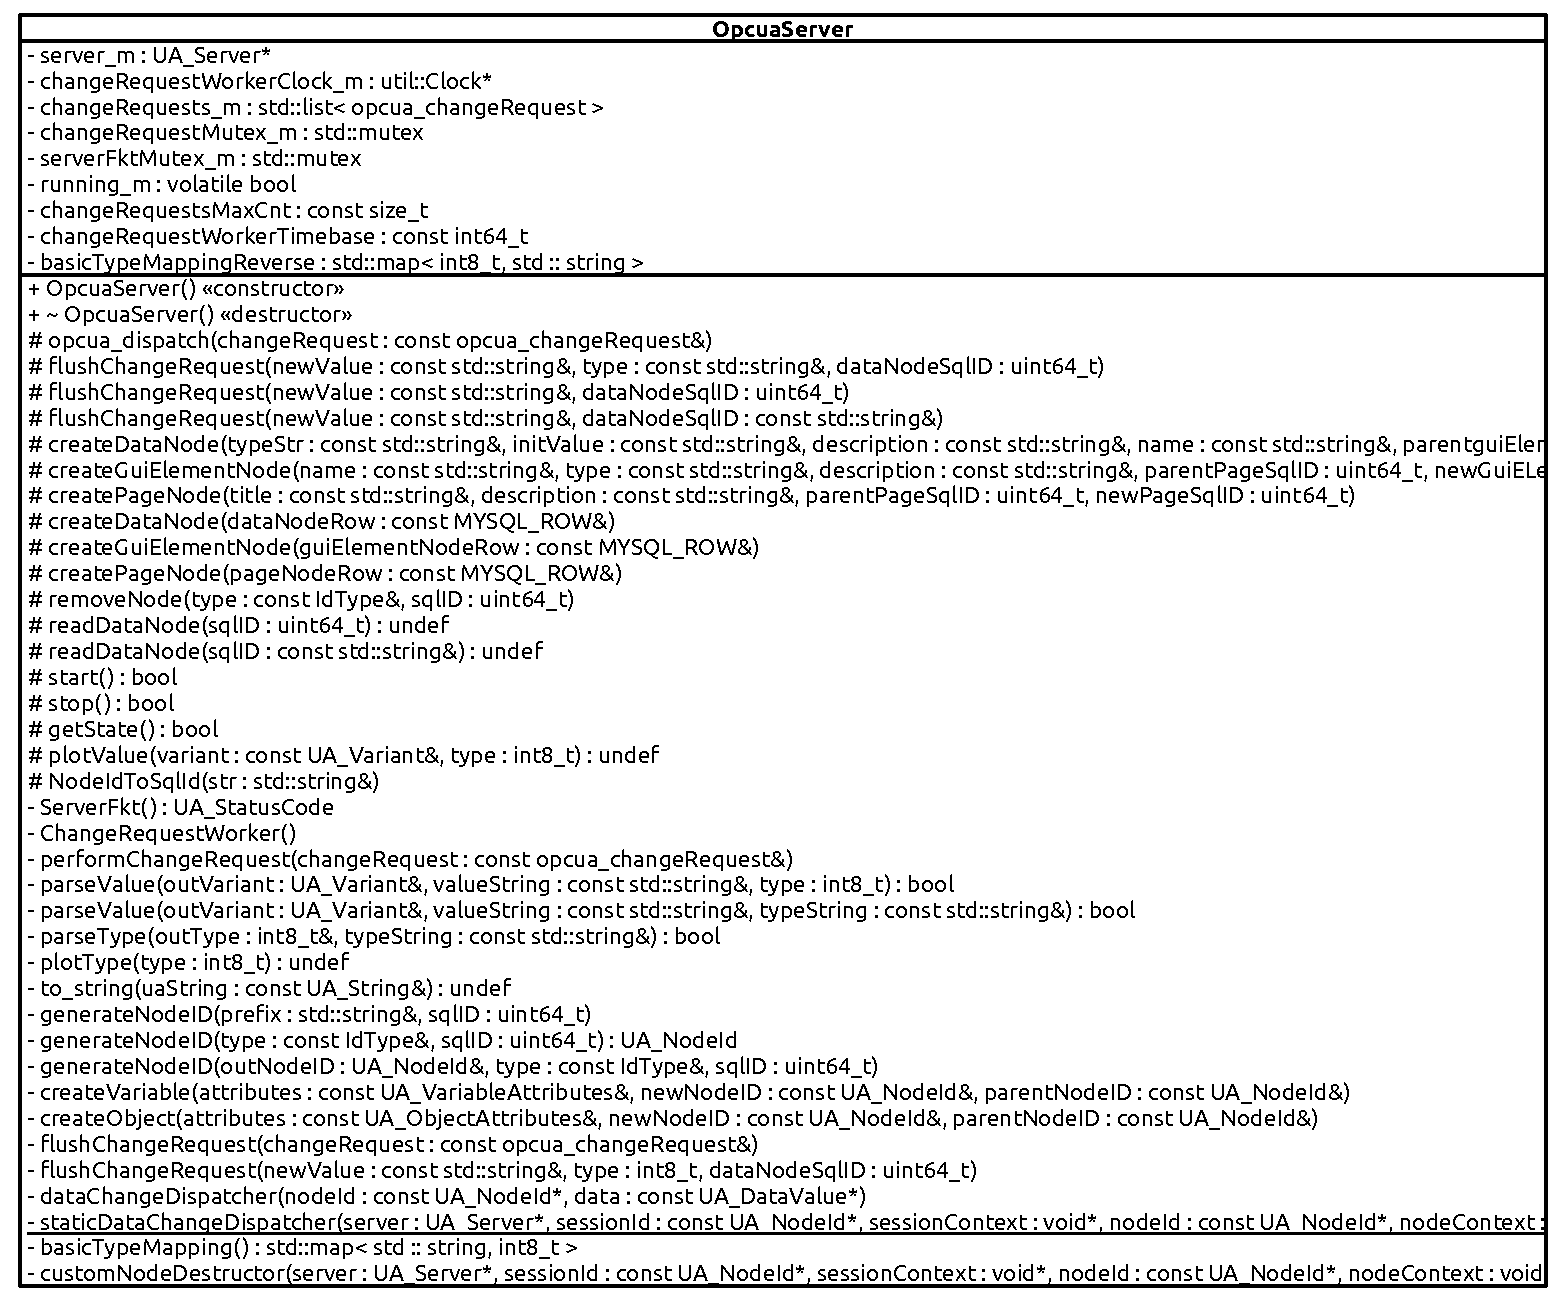
\includegraphics[width=\textwidth]{content/hauptteil/umsetzungPoC/backend/uml/classesOfOverview/OpcuaServer.pdf}
  \caption{Klassediagramm der Klasse OpcuaServer}
  \label{fig:backend:classDiag:OpcuaServer}
\end{figure}
%beschreibung msg klasse mit diagram
\begin{figure}[ht]
  \centering
  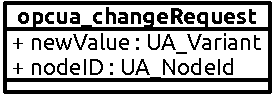
\includegraphics[width=0.2\textwidth]{content/hauptteil/umsetzungPoC/backend/uml/classesOfOverview/opcua_changeRequest.pdf}
  \caption{Klassediagramm der Klasse opcua\_changeRequest}
  \label{fig:backend:classDiag:opcuaCR}
\end{figure}
%dispatcher codeausschnitt
%beschreibung dispatcher




%%%%BRAINSTORM BABU:
%packete zeigen, beispiele aktionen screenshot chrome wss